% Figure "hinge" of "Galashin's Conjecture 4.3 via a convex gradient": the points v_r = e^{2i theta_r} on the unit circle
% and, for each crossing edge e=(p,q), the chord |v_q - v_p| = 2 sin(delta_e) (Lemma on the hinge identity, CLH-1).
% Source in the paper's own fonts (T1, Latin Modern, 11pt) at the text width (6.5in = 468bp), so \includegraphics does not
% rescale it. Illustrates the claim rows of the hinge identity; it adds no assertion.
% Every value drawn is read from Lean output lines (SHA-256 of the lines):
%   picture D73  9aa699420e1762fcebbb22d5ecc8ae985905c5a3e6e8005c32b668ed1784dcd2   (angles theta/pi = (0,0.1,0.7,0.3,0.8))
% The combinatorial data (crossing edges of Conj43.crossEdges for the window (3,5,1,2,4)) are Lean values; the angles,
% gaps delta_e and chord lengths are floating-point values of Lean code that follows the paper's formulas.
% Build: pdflatex <this file> && pdftocairo -svg <this file>.pdf <this file>.svg
\documentclass[11pt]{standalone}
\usepackage[T1]{fontenc}
\usepackage{lmodern}
\usepackage{amsmath,amssymb}
\usepackage{tikz}
\usetikzlibrary{arrows.meta,positioning,calc}

% the palette of the paper's other figures: blue solid for the first strand, cycle or arc, ochre dashed for the second
\definecolor{ink}{HTML}{233740}
\definecolor{muted}{HTML}{65757D}
\definecolor{pblue}{HTML}{0072B2}
\definecolor{qochre}{HTML}{B87827}

\tikzset{
  base/.style={draw=muted, line width=0.5pt},
  ttl/.style={font=\small, text=ink, inner sep=0pt},
  lab/.style={font=\footnotesize, inner sep=1.2pt, text=ink},
  labm/.style={font=\small, inner sep=1.2pt, text=ink},
  labP/.style={font=\small, inner sep=1.2pt, text=pblue},
  labQ/.style={font=\small, inner sep=1.2pt, text=qochre},
  idx/.style={font=\footnotesize, text=muted, inner sep=0pt},
  negE/.style={font=\small, text=pblue, inner sep=0pt},
  posE/.style={font=\small, text=qochre, inner sep=0pt},
  zeroE/.style={font=\small, text=muted, inner sep=0pt},
  vtx/.style={circle, draw=ink, fill=white, line width=0.6pt, inner sep=0pt, minimum size=16bp, font=\small, text=ink},
  cycP/.style={pblue, line width=1.1pt, -{Stealth[length=5pt,width=4.2pt]}, shorten >=1pt, shorten <=1pt},
  cycQ/.style={qochre, line width=1.1pt, dash pattern=on 4pt off 1.6pt, -{Stealth[length=5pt,width=4.2pt]}, shorten >=1pt, shorten <=1pt},
  chord/.style={pblue, line width=0.9pt},
  arrP/.style={pblue, line width=1.0pt, -{Stealth[length=4.4pt,width=3.8pt]}},
  arrQ/.style={qochre, line width=1.0pt, dash pattern=on 4pt off 1.6pt, -{Stealth[length=4.4pt,width=3.8pt]}},
  arrM/.style={muted, line width=0.6pt, -{Stealth[length=4pt,width=3.4pt]}},
}

\begin{document}
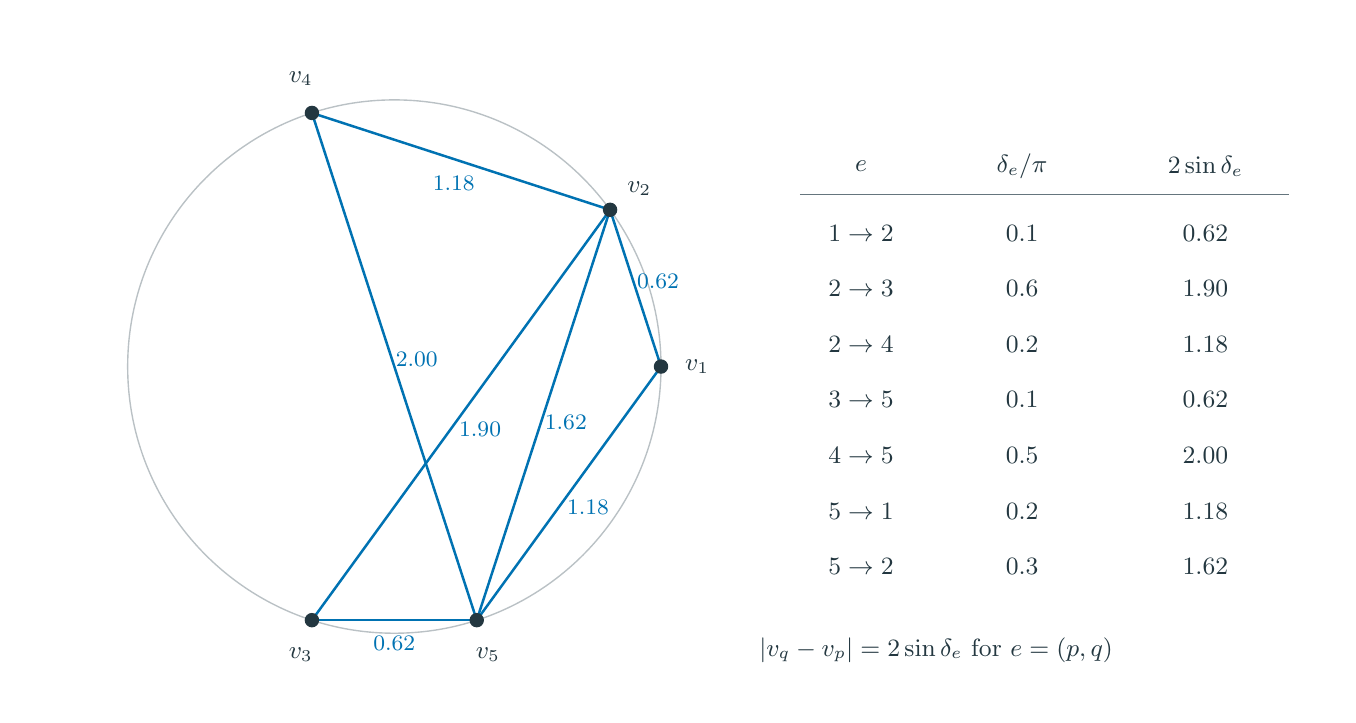
\begin{tikzpicture}[x=1bp,y=1bp]
\useasboundingbox (0,0) rectangle (468.000,240.000); %@ hinge canvas w=468.000 h=240.000
\draw[draw=muted!45, line width=0.5pt] (132.000,118.000) circle (96.000bp); %@ hinge circle cx=132.000 cy=122.000 R=96.000
\draw[chord] (228.000,118.000) -- (209.666,174.427); %@ hinge chord p=1 q=2 len=0.62
\draw[chord] (209.666,174.427) -- (102.334,26.699); %@ hinge chord p=2 q=3 len=1.90
\draw[chord] (209.666,174.427) -- (102.334,209.301); %@ hinge chord p=2 q=4 len=1.18
\draw[chord] (102.334,26.699) -- (161.666,26.699); %@ hinge chord p=3 q=5 len=0.62
\draw[chord] (102.334,209.301) -- (161.666,26.699); %@ hinge chord p=4 q=5 len=2.00
\draw[chord] (161.666,26.699) -- (228.000,118.000); %@ hinge chord p=5 q=1 len=1.18
\draw[chord] (161.666,26.699) -- (209.666,174.427); %@ hinge chord p=5 q=2 len=1.62
\node[lab,text=pblue] at (226.917,148.840) {$0.62$}; %@ hinge chordlabel p=1 q=2 val=0.62
\node[lab,text=pblue] at (162.877,95.567) {$1.90$}; %@ hinge chordlabel p=2 q=3 val=1.90
\node[lab,text=pblue] at (153.373,183.780) {$1.18$}; %@ hinge chordlabel p=2 q=4 val=1.18
\node[lab,text=pblue] at (132.000,18.199) {$0.62$}; %@ hinge chordlabel p=3 q=5 val=0.62
\node[lab,text=pblue] at (140.084,120.627) {$2.00$}; %@ hinge chordlabel p=4 q=5 val=2.00
\node[lab,text=pblue] at (201.709,67.353) {$1.18$}; %@ hinge chordlabel p=5 q=1 val=1.18
\node[lab,text=pblue] at (193.750,97.936) {$1.62$}; %@ hinge chordlabel p=5 q=2 val=1.62
\fill[ink] (228.000,118.000) circle (2.6bp); %@ hinge point r=1
\node[labm] at (241.000,118.000) {$v_1$}; %@ hinge pointlabel r=1
\fill[ink] (209.666,174.427) circle (2.6bp); %@ hinge point r=2
\node[labm] at (220.183,182.069) {$v_2$}; %@ hinge pointlabel r=2
\fill[ink] (102.334,26.699) circle (2.6bp); %@ hinge point r=3
\node[labm] at (98.317,14.335) {$v_3$}; %@ hinge pointlabel r=3
\fill[ink] (102.334,209.301) circle (2.6bp); %@ hinge point r=4
\node[labm] at (98.317,221.665) {$v_4$}; %@ hinge pointlabel r=4
\fill[ink] (161.666,26.699) circle (2.6bp); %@ hinge point r=5
\node[labm] at (165.683,14.335) {$v_5$}; %@ hinge pointlabel r=5
\node[labm] at (300.000,190.000) {$e$}; %@ hinge head col=e
\node[labm] at (358.000,190.000) {$\delta_e/\pi$}; %@ hinge head col=delta
\node[labm] at (424.000,190.000) {$2\sin\delta_e$}; %@ hinge head col=len
\draw[muted, line width=0.4pt] (278.000,180.000) -- (454.000,180.000);
\node[labm] at (300.000,166.000) {$1\to2$}; %@ hinge row i=1 p=1 q=2
\node[labm] at (358.000,166.000) {$0.1$}; %@ hinge rowdelta i=1 val=0.1
\node[labm] at (424.000,166.000) {$0.62$}; %@ hinge rowlen i=1 val=0.62
\node[labm] at (300.000,146.000) {$2\to3$}; %@ hinge row i=2 p=2 q=3
\node[labm] at (358.000,146.000) {$0.6$}; %@ hinge rowdelta i=2 val=0.6
\node[labm] at (424.000,146.000) {$1.90$}; %@ hinge rowlen i=2 val=1.90
\node[labm] at (300.000,126.000) {$2\to4$}; %@ hinge row i=3 p=2 q=4
\node[labm] at (358.000,126.000) {$0.2$}; %@ hinge rowdelta i=3 val=0.2
\node[labm] at (424.000,126.000) {$1.18$}; %@ hinge rowlen i=3 val=1.18
\node[labm] at (300.000,106.000) {$3\to5$}; %@ hinge row i=4 p=3 q=5
\node[labm] at (358.000,106.000) {$0.1$}; %@ hinge rowdelta i=4 val=0.1
\node[labm] at (424.000,106.000) {$0.62$}; %@ hinge rowlen i=4 val=0.62
\node[labm] at (300.000,86.000) {$4\to5$}; %@ hinge row i=5 p=4 q=5
\node[labm] at (358.000,86.000) {$0.5$}; %@ hinge rowdelta i=5 val=0.5
\node[labm] at (424.000,86.000) {$2.00$}; %@ hinge rowlen i=5 val=2.00
\node[labm] at (300.000,66.000) {$5\to1$}; %@ hinge row i=6 p=5 q=1
\node[labm] at (358.000,66.000) {$0.2$}; %@ hinge rowdelta i=6 val=0.2
\node[labm] at (424.000,66.000) {$1.18$}; %@ hinge rowlen i=6 val=1.18
\node[labm] at (300.000,46.000) {$5\to2$}; %@ hinge row i=7 p=5 q=2
\node[labm] at (358.000,46.000) {$0.3$}; %@ hinge rowdelta i=7 val=0.3
\node[labm] at (424.000,46.000) {$1.62$}; %@ hinge rowlen i=7 val=1.62
\node[labm,anchor=west] at (262.000,16.000) {$\lvert v_q-v_p\rvert=2\sin\delta_e$ for $e=(p,q)$}; %@ hinge note
\end{tikzpicture}
\end{document}
